\documentclass[english]{article}

\usepackage{babel}
\usepackage{graphicx}
\usepackage{times}
\usepackage{pifont}
\usepackage[margin=1in]{geometry}
\usepackage{eurosym}
\usepackage{fancyhdr}
\usepackage{wrapfig}

\pagestyle{fancy}
\fancyhf{}

%HEADER
%**************************************************************************************
\lhead{Functions and Triggers}		 	 
\rhead{Database Server} 
%**************************************************************************************

\date{}
\setlength\parindent{0pt}

\begin{document}

\title{\vspace{2in}Functions and Triggers\\ PL/pgSQL\\
\small for Database Server\\
\vspace{0.5in}
\includegraphics{savonia.jpg}}

\nopagebreak
\maketitle


\vspace{3in}

\author{
\begin{flushright}
Alexey Tukalo,\\
EFA12SF,\\
Information Technology,\\
Savonia University of Applied Sciences
\end{flushright}
}

\date{\today}
\thispagestyle{empty}

\newpage
\setcounter{page}{1}
\setcounter{tocdepth}{2}
\tableofcontents

\newpage

%MAIN CONTENT ******************************************************************************************************************

\section{Logg table, function and triggers for it}
\subsection{Logg table}
I have create the Logg table with three columns:

\begin{enumerate}
\item ID - integer Primery Key
\item When - date
\item Description - character varying 
\end{enumerate}


It was created by script on the picture 1.

\begin{figure}[hb]
\centerline{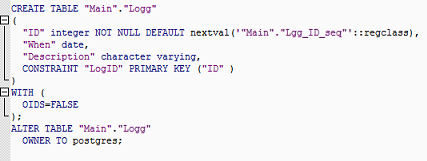
\includegraphics{PLPGSQL/LoggScript}}
\caption{Script for Logg table}
\end{figure}


And the table itself is displayed on the figure 2.


\begin{figure}[hb]
\centerline{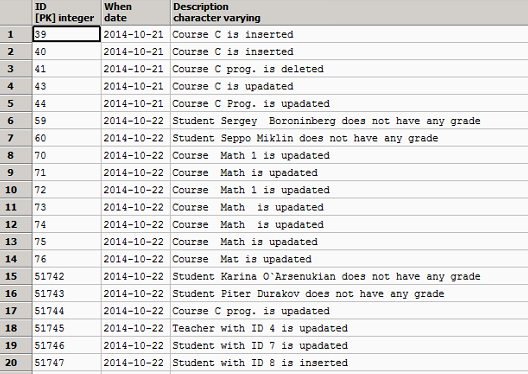
\includegraphics{PLPGSQL/LoggTable}}
\caption{Logg table}
\end{figure}

\subsection{Function badStudents()}
After that I have written the code for the function which return amount of students without any accepted course, also it insets a row per student into the Logg table, the description field may look like this "Student XX YY does not have any grades". You can see the code and output of the function on the figures below.

\begin{figure}[h]
\centerline{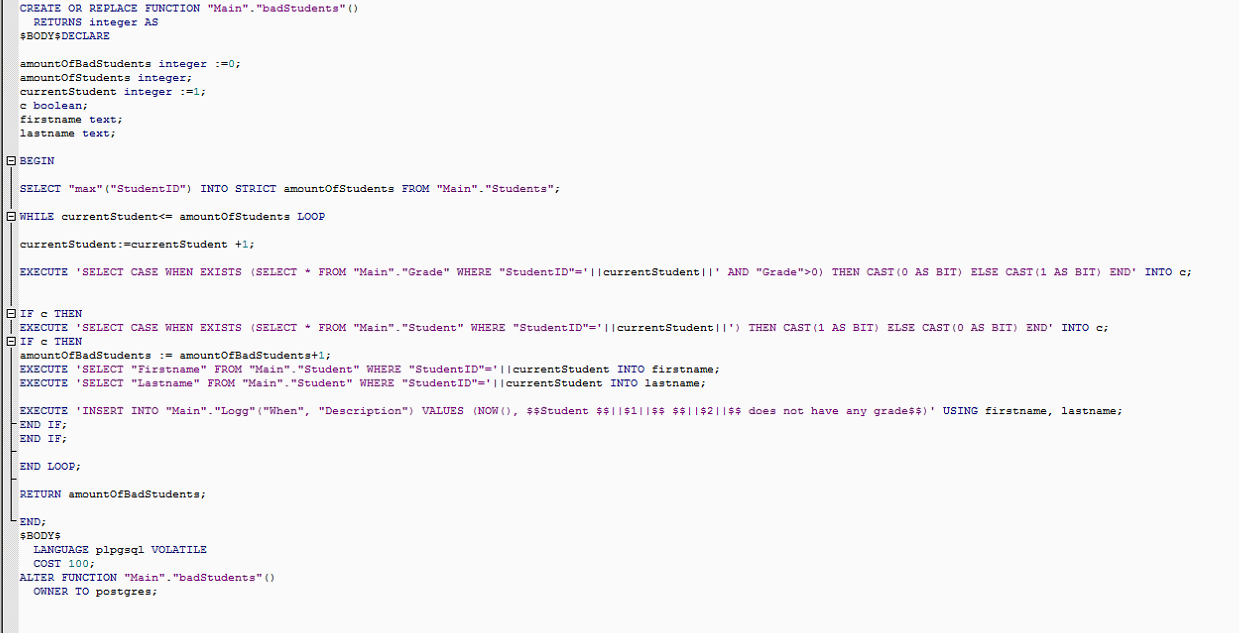
\includegraphics[scale=0.6]{PLPGSQL/badStudentScript}}
\caption{Code of badStudents()}
\end{figure}

\begin{figure}[h]
\centerline{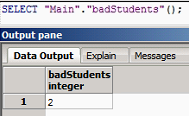
\includegraphics{PLPGSQL/badStudentOutPut}}
\caption{badStudents() output}
\end{figure}

After the execution of the function it also added rows number 15 and 16 on the Logg table, look at picture 2.
\subsection{edited()}
I also made a trigger edited() which inserts a row into the logg table if course information is inserted/updated/deleted.  The content of the description field may look like this " Course ZZZ is inserted/deleted/updated". The output of the trigger you can find on the figure 2.
\begin{figure}[h]
\centerline{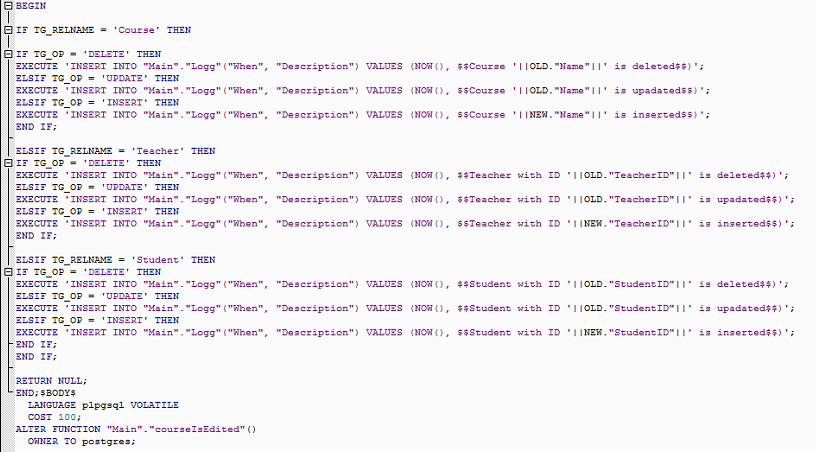
\includegraphics[scale=0.8]{PLPGSQL/editSource}}
\caption{edited() source code}
\end{figure}

\section{Archived column and function for it}
\subsection{Archived column}
After that I have added new column for Student table, the column is selected on the 6th picture. 

\begin{figure}[h]
\centerline{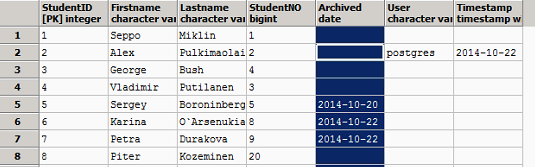
\includegraphics{PLPGSQL/ArchivedStudentTable}}
\caption{Student Table with Archived column}
\end{figure}
\subsection{Function archived()}
At the next step I have written the code below and after the execution the function added dates into rows from 5th to 7th on the column Archived.

\begin{figure}[h]
\centerline{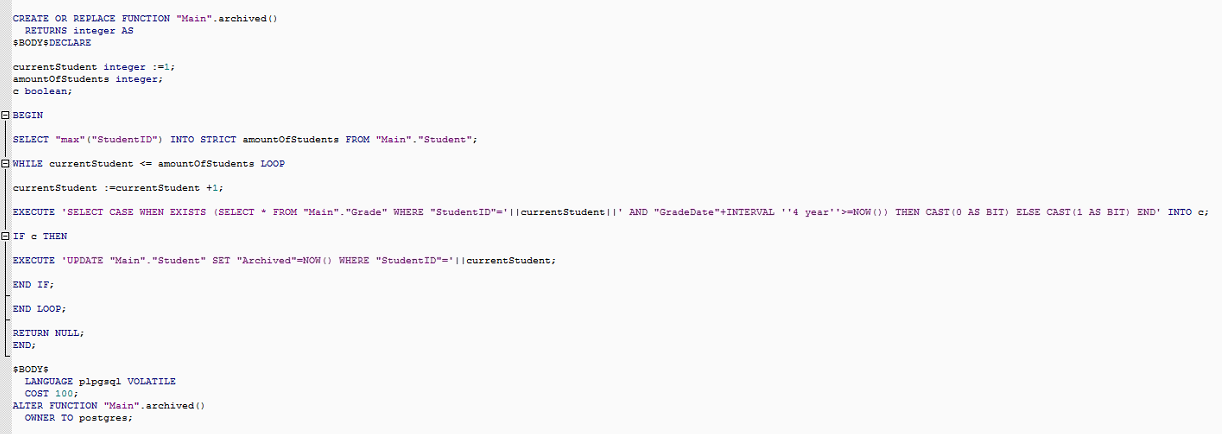
\includegraphics[scale=0.6]{PLPGSQL/ArchivedFunction}}
\caption{Source code for archived()}
\end{figure}

\section{Timestamp and User columns}
I have added the columns for Timestamp and User for tables Course, Teacher, Student. And the trigger code you can see on the picture 8. The result of the code is represented on the 9th figure.


\begin{figure}[h!]
\centerline{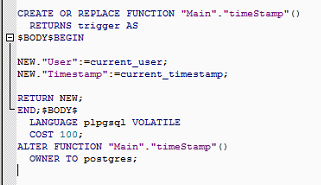
\includegraphics{PLPGSQL/SourceTimeStamp}}
\caption{timeStamp() source code}
\end{figure}
\centerline{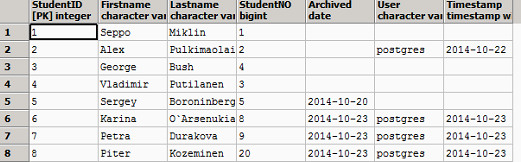
\includegraphics{PLPGSQL/studentTable}}
\begin{figure}[h!]

\centerline{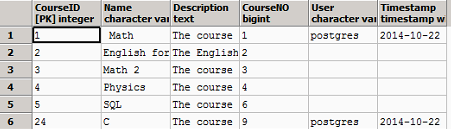
\includegraphics{PLPGSQL/courseTable}}
\centerline{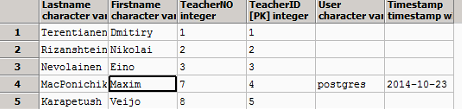
\includegraphics{PLPGSQL/teacherTable}}
\caption{Tables with the columns}
\end{figure}
\newpage

\section{Student protection}
The last task asked to make the trigger which protects students with accepted courses from deleting. The function has to check it via query and show error message if it is impossible to delete the student, picture 10.
\begin{figure}[h!]
\centerline{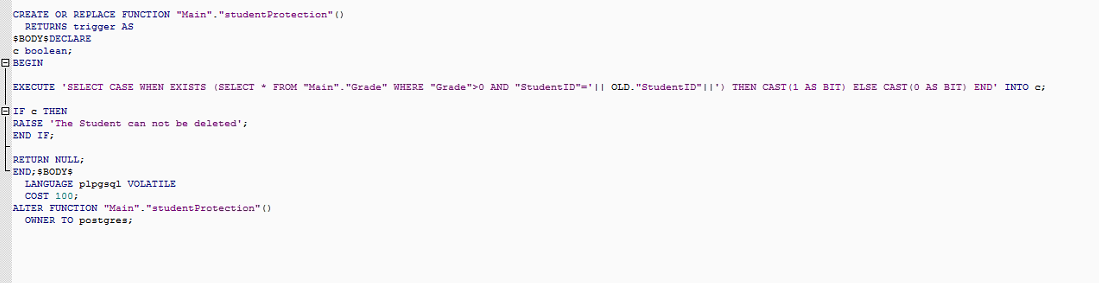
\includegraphics[scale=0.7]{PLPGSQL/studentProtectionSource}}
\caption{studentProtection() source code}
\end{figure}
\begin{figure}[h!]
\centerline{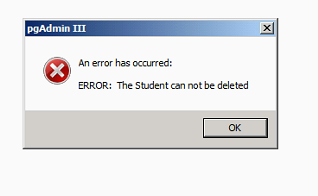
\includegraphics[scale=0.9]{PLPGSQL/errorDeleting}}
\caption{studentProtection() Error message}
\end{figure}

\end{document}
